\chapter{Переменные Лагранжа и Эйлера для описания движения частицы сплошной
среды. Вектор смещения. Тензор смещения как сумма тензора деформации и тензора
поворота.}

Лагранж предложил выделить в сплошной среде отдельные точки и следить за их
движением. Координаты которыми характеризуется данная точка и не меняются при
её движении носят название \emph{переменных Лагранжа}. В качестве таких
координат можно выбрать положения точки в начальный момент времени \( \xi^i \)
или её цвет если все точки сплошной среды окрашены в разные цвета.
Закон движения каждой точки в переменных Лагранжа имеет вид
\[
    \vec{r} = \vec{r}(\xi^i, t)
\] 
или в контрвариантных криволинейных координатах \( q^j \)
\[
    q^j = q^j(\xi^i, t).
\]
Скорость по Лагранжу -- скорость движения данной частицы, для неё
\( \xi^i~=~const \):
\[
    \left.\der{\vec{r}}{t}\right|_{\xi^i = const} = \pder{\vec{r}}{t}.
\]
Ускорение по Лагранжу   
\[
    \left.\dder{\vec{r}}{t}\right|_{\xi^i = const} = \ppder{\vec{r}}{t}.
\]
        
Эйлер предложил не следить за каждой отдельной частицей, а следить за данной
точкой пространства измеряя скорости, пролетающих через неё частиц и фиксируя
их вид. Криволинейные координаты данной точки \( q^j \)  и время \( t \) носят
название \emph{переменных Эйлера}.

Выражение для радиус-вектора частицы \( \vec{r} = \vec{r}(\xi^i, t) \) и
компонент радиус-вектора частицы \( q^j = q^j (\xi^i, t) \) позволяет выяснить,
какие частицы проходят через данную точку: \( \xi^i = \xi^i(q^j, t) \).
Скорость по Эйлеру -- скорость в данной точке \( \vec{r}_{M} \):
\[
    \der{\vec{r}}{t} = 
    \left.\pder{\vec{r}}{t}\right|_{\xi^i = \xi^i(\vec{r}_{M}, t)} +
    \left.\pder{\vec{r}}{\xi^i}
    \der{\xi^i}{t}\right|_{\xi^i = \xi^i(\vec{r}_{M}, t)} =
    \left.\pder{\vec{r}}{t}\right|_{\xi^i = \xi^i(\vec{r}_{M}, t)} +
    \left.\pder{\vec{r}}{\xi^i}
    \pder{\xi^i}{t}\right|_{\xi^i = \xi^i(\vec{r}_{M}, t)}
\]
Ускорение по Эйлеру
\[
    \dder{\vec{r}}{t}.
\]

Также иногда вводят перемещение по Эйлеру. \emph{В курсе Лурье} это разность
между конечным и начальным радиус-вектором. Определяя переменные Лагранжа как
координаты радиус-вектора в начальный момент времени и полагая, что наша
система координат не связана с точками сплошной среды (а бывает и такое), для
перемещений по Эйлеру можно записать: \( s^i = q^i - \xi^i \).
    
Рассмотрим две близкие частицы сплошной среды \( A \) и \( B \) в момент
времени \( t \), в следующий момент времени \( t+dt \) они сместятся на
некоторые векторы \( \vec{s}_{A} \), \( \vec{s}_{B} \):
\begin{gather*}
    \vec{s}_{A} = \vec{r}_{A}(t+dt) -\vec{r}_{A}(t),\\
    \vec{s}_{B} = \vec{r}_{B}(t+dt) -\vec{r}_{B}(t).
\end{gather*}
Полагая что координаты вектора \( \vec{r}_{B} - \vec{r}_{A} \) равные в
криволинейных координатах \( \delta q^i \) малы, в первом приближении:
\[
    \vec{s}_{B} - \vec{s}_{A} = \pder{ \vec{s}_{A}}{q^i}\delta q^i 
    = \nabla_i s^j \delta q^i,
\]
\( s^j \) контрвариантные компоненты вектора \( \vec{s}_{A} \).

Вектор \( s^j \) носит название \emph{вектора смещения}. Он показывает, как
сместилась бы частица при поступательном движении будь она частицей твёрдого
тела.

\emph{Тензором смещения} называется тензор \( b^j_{i} = \nabla_i s^j \) или
соответствующий ему ковариантный тензор \( b_{ki} = g_{jk}\nabla_i s^j \).
Тензор смещения можно представить, как и всякий тензор второго ранга, в виде
суммы симметричного и антисимметричного тензоров:
\[
    b^j_{i} = 
    \underbrace{\frac{1}{2} (b^j_{i}+b^j_{i})}_{\substack{= e^j_{i} \\
    \text{симметричный}
    }} \ \ \ + 
    \underbrace{\frac{1}{2} (b^j_{i}-b^j_{i}).}_{\substack{= \phi^j_{i}\\
    \text{антисимметричный}
    }}
\]
Тогда 
\[
    s^j_B = s^j_A + e^j_{i}\delta q^i + \phi^j_{i}\delta q^i.
\]
\sidefig(7cm)
{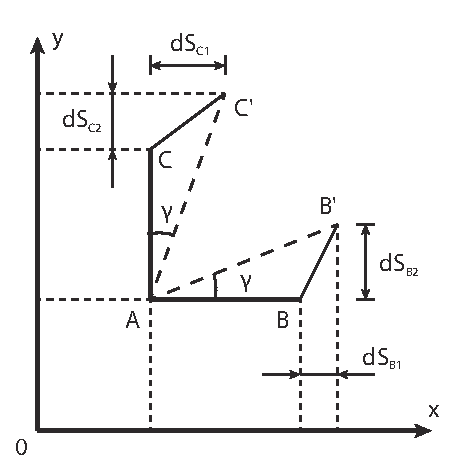
\includegraphics[width=\textwidth]{08}}
{Определим физический смысл тензоров \( e^j_{i} \), \( \phi^j_{i} \).
Рассмотрим плоскую сплошную среду в декартовых координатах \( (x, y) \) или
\( (x^1, x^2) \) как показано на рисунке справа. Выделим в ней два бесконечно
малых стержня \( AB \) и \( AC \). Декартову систему координат привяжем к точке
\( A \) и рассмотрим малые по сравнению со стержнями перемещения точек \( B \)
и \( C \) в точки \( B' \) и \( C' \).}

В декартовых координатах ковариантная производная переходит в частную,
обозначив длины стержней \( AB \) и \( AC \) \( \delta x \) и \( \delta y \)
соответственно, получим:
    \begin{gather*}
    e^1_{1} = \pder{s^1}{x^1} = \frac{ds_{_{B1}}}{\delta x} 
    \text{   - относительная деформация стержня AB,} \\
    e^1_{2} = \pder{s^1}{x^2} = \frac{ds_{_{C1}}}{\delta y} 
    \text{   - поворот(сдвиг) стержня AB на }\gamma, \\
    e^2_{1} = \pder{s^2}{x^1} = \frac{ds_{_{B2}}}{\delta x} 
    \text{   - поворот(сдвиг) стержня AC на }\gamma, \\  
    e^2_{2} = \pder{s^2}{x^2} = \frac{ds_{_{C2}}}{\delta y} 
    \text{   - относительная деформация стержня AC.}
    \end{gather*}
    
Таким образом тензор \( e^j_{i} \) - \textit{тензор деформации}.

Тензор \( \phi^j_{i} \) - антисимметричный, поэтому свёртку
\( \phi^j_{i}\delta q^i \) можно заменить векторным произведением:
\[
    \phi^j_{i}\delta q^i = \vec{\Phi} \times \delta\vec{s}.
\]
Если вспомнить понятие вектора поворота, видно, что это \( \vec{\Phi} \).
Тензор \( \phi^j_{i} \) носит название \emph{тензора поворота}.

\textbf{Теорема Гельмгольца}\\
\textit{Движение малой частицы среды в каждый момент времени представляет
собой поступательное движение вместе с полюсом (точкой внутри малой частицы),
сферическое движение вокруг полюса и движение деформации.}

\newpage
